\documentclass[9pt]{beamer}

%~~~~~~~~~~~~~~~~~~~~~~~~~~~~~~~~~~~~~~~~~~~~~~~~~~~~~~~~~~~~~~~~~~~~~~~~~~~~~~
% Use roboto Font (recommended)
\usepackage[sfdefault]{roboto}
\usepackage[utf8]{inputenc}
\usepackage[T1]{fontenc}
%~~~~~~~~~~~~~~~~~~~~~~~~~~~~~~~~~~~~~~~~~~~~~~~~~~~~~~~~~~~~~~~~~~~~~~~~~~~~~~

%~~~~~~~~~~~~~~~~~~~~~~~~~~~~~~~~~~~~~~~~~~~~~~~~~~~~~~~~~~~~~~~~~~~~~~~~~~~~~~
% Define where theme files are located. ('/styles')
\usepackage{styles/fluxmacros}
\usefolder{styles}
% Use Flux theme v0.1 beta
% Available style: asphalt, blue, red, green, gray 
\usetheme[style=green]{flux}
%~~~~~~~~~~~~~~~~~~~~~~~~~~~~~~~~~~~~~~~~~~~~~~~~~~~~~~~~~~~~~~~~~~~~~~~~~~~~~~

%~~~~~~~~~~~~~~~~~~~~~~~~~~~~~~~~~~~~~~~~~~~~~~~~~~~~~~~~~~~~~~~~~~~~~~~~~~~~~~
% Extra packages for the demo:
\usepackage{booktabs}
\usepackage{colortbl}
\usepackage{ragged2e}
\usepackage{schemabloc}
\usepackage{subfigure}
\usepackage{hyperref}
\usepackage[usenames]{color}
%~~~~~~~~~~~~~~~~~~~~~~~~~~~~~~~~~~~~~~~~~~~~~~~~~~~~~~~~~~~~~~~~~~~~~~~~~~~~~~
%~~~~~~~~~~~~~~~~~~~~~~~~~~~~~~~~~~~~~~~~~~~~~~~~~~~~~~~~~~~~~~~~~~~~~~~~~~~~~~
% Informations
\subtitle{\\
\LARGE{CAsimulations: Modelación de dinámicas topológicas } \\
\LARGE{en la propagación de una enfermedad usando}\\
\LARGE{autómatas celulares}}
%\subtitle{The winding number}
\author{Jorge Andres Ibañez Huertas, 
Carlos Isaac Zainea Maya}
\institute{Central University, Bogotá}
\date{\today}
\titlegraphic{Imagenes/logo.png}
%~~~~~~~~~~~~~~~~~~~~~~~~~~~~~~~~~~~~~~~~~~~~~~~~~~~~~~~~~~~~~~~~~~~~~~~~~~~~~~

\begin{document}

% Generate title page
\titlepage

\begin{frame}{Introducción}
Hoy en día existen distintos modelos matemáticos para proyectar el progreso de una enfermedad con el objetivo de brindar estrategias de control y de prevención \cite{epiDictionary}. Contingencias como la vivida con el COVID 19 promueven una mayor comprensión y planteamiento de estos modelos desde diferentes perspectivas.

Hemos identificado dos grupos de modelos: los que están basados en compartimientos y los modelos de aprendizaje. Entre los cuales cabe destacar que a pesar de su capacidad de predicción, se dejan de lado comportamientos espaciales y en ocasiones la implementación puede estar limitada por la naturaleza de los datos.

Hemos identificado que la gran mayoría de los modelos describen la propagación asumiendo comportamientos en masa como por ejemplo el desplazamiento entre regiones de un país \cite{populationDensity} y esto nos motiva a preguntarnos por \textbf{¿cuál es el nivel de incidencia de las interacciones sociales en la propagación de una enfermedad?}

\end{frame}

\begin{frame}{Objetivos}
\begin{enumerate}
    \item Crear una herramienta que permita analizar la propagación de una enfermedad en función de las interacciones sociales individuales.
    \item Proporcionar una metodología para formular modelos epidemiológicos basados en agentes a partir de patrones y reglas lógicas.
    \item Determinar el impacto de las interacciones sociales en la propagación de una enfermedad.
\end{enumerate}
\end{frame}

\begin{frame}
\frametitle{Tabla de Contenidos}
\tableofcontents
\end{frame}

\section{Preliminares}

\subsection{Modelos compartimentales: Modelos SIS y SIR}
\begin{frame}{Modelos compartimentales}
Tradicionalmente, se han utilizado modelos de compartimientos para elaborar análisis epidemiológicos. En estos modelos, cada individuo perteneciente a la población de estudio, es clasificado en uno de $n$ posibles ''compartimientos'', según su estado de salud.

Generalmente, se consideran tres estados en las que podemos dividir a la población en el tiempo: Los que pueden contraer la enfermedad, los que se infectan y los que se recuperan. Los modelos que consideran estas variaciones se conocen como los modelos SIS y SIR.

\textbf{Nota:} Usaremos las versiones con tamaño de población constante de los modelos SIS y SIR. Se espera que en futuras investigaciones se profundice en poblaciones de tamaño variable.
\end{frame}

\begin{frame}{Modelos compartimentales: Modelos SIS y SIR}
\begin{minipage}{0.55\textwidth}
\centering{El modelo SIS}
\begin{figure}[h]
  \centering
    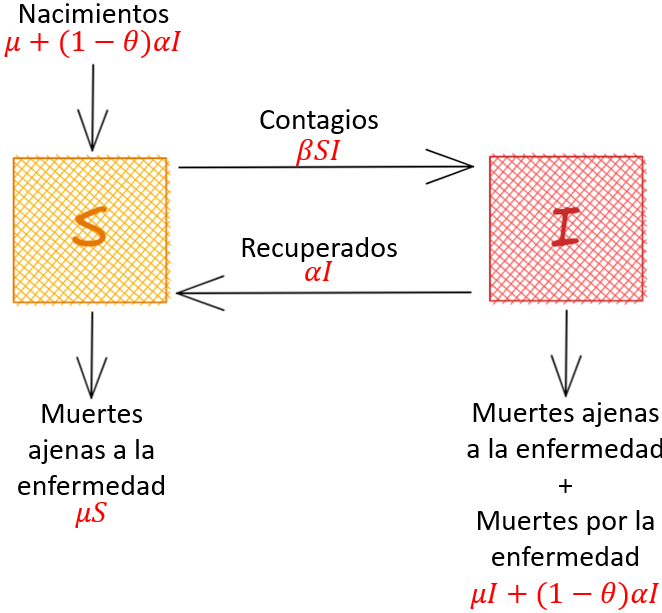
\includegraphics[width=0.65\textwidth]{Imagenes/SIS_compartimientos.PNG}
\end{figure}
\centering{El modelo SIR}
\begin{figure}[h]
  \centering
    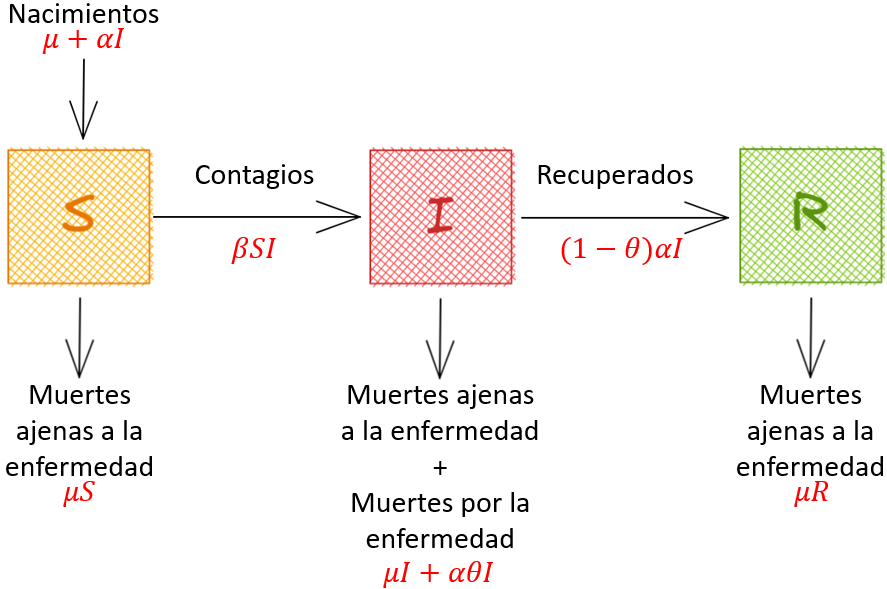
\includegraphics[width=0.8\textwidth]{Imagenes/SIR_compartimientos.PNG}
\end{figure}
\end{minipage}
\hfill
\begin{minipage}{0.415\textwidth}
\begin{block}{\textbf{Parámetros de los modelos SIS y SIR}}
\begin{itemize}
    \item \textbf{Tasa de infección $\beta$:} Probabilidad que tiene un individuo susceptible de adquirir la enfermedad luego de tener contacto con un infectado.
    \item \textbf{Tasa de recuperación $\alpha$:} Probabilidad de que un infectado se recupere de la enfermedad. En ocasiones representa el tiempo medio que tarda un infectado en recuperarse de la enfermedad \cite{diego2010}.
    \item \textbf{Tasa de natalidad/mortalidad $\mu$.}
    \item \textbf{Tasa de muerte por enfermedad $\theta$.}
\end{itemize}
\end{block}
\end{minipage}
\end{frame}

\subsection{Autómatas celulares y topología}
\begin{frame}{Autómatas celulares y topología}
% Podemos pensar en un autómata celular como un conjunto de células que tienen diferentes comportamientos en el tiempo y que interactúan entre sí, de la misma manera que en sistema biológico de donde se obtiene su nombre.

\begin{figure}[h]
  \centering
    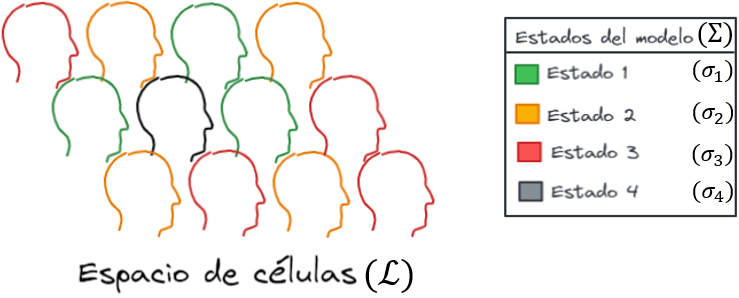
\includegraphics[width=0.7\textwidth]{Imagenes/espacioYEstados.png}
\end{figure}

% Un \textbf{espacio de células} $\mathcal{L}$ es el conjunto donde viven e interactúan todas las células que se consideran para el modelo. En general este espacio es discreto, regular y finito.%, esto último debido a las limitaciones computacionales presentes en las herramientas con las que se construyen los modelos en autómatas celulares.

% El \textbf{conjunto de estados} $\Sigma$ es el conjunto finito de todas las posibles categorías en las que pueden estar las células del espacio $\mathcal{L}$. %Cada elemento $\sigma$ de $\Sigma$ será conocido como un estado del modelo.

Las \textbf{reglas} que rigen el comportamiento de los estados de las células depende del estado de sus vecinos. Se deben aplicar en simultáneo sobre cada una de las células.
\end{frame}

\begin{frame}{Autómatas celulares y topología}
\begin{figure}[h]
  \centering
    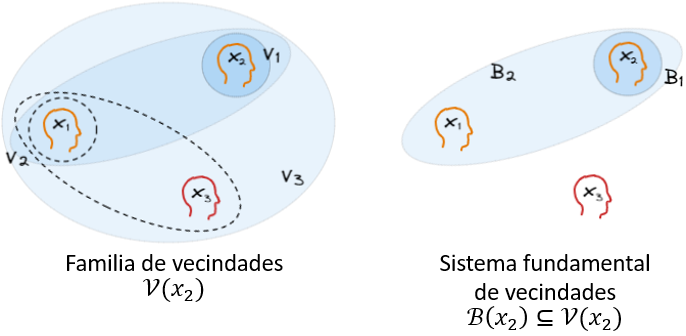
\includegraphics[width=0.8\textwidth]{Imagenes/vecindadesDiagrama.png}
\end{figure} 
Vecindades usuales:
\begin{figure}[h]
  \centering
    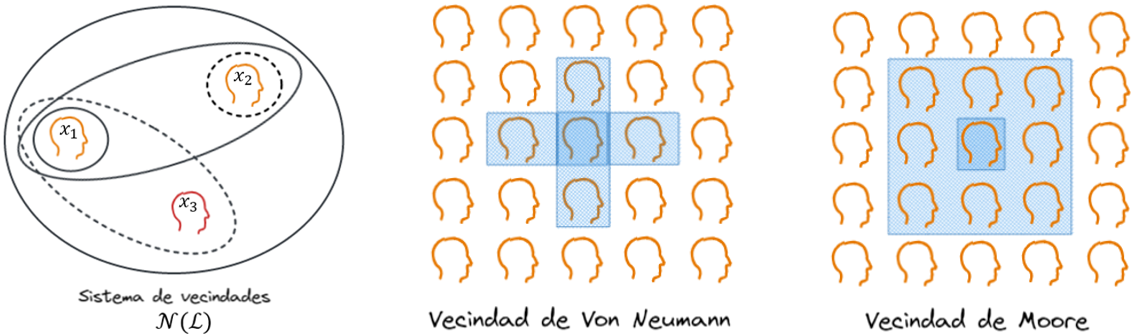
\includegraphics[width=0.45\textwidth]{Imagenes/vecindadesMyVN.png}
\end{figure} 
\textbf{Definición:} Un espacio topológico $X$ que tiene un sistema fundamental de vecindades numerable en cada uno de sus puntos se dice que satisface el primer axioma de numerabilidad o simplemente que es uno-numerable.
\end{frame}

\section{Modelos epidemiológicos en autómatas celulares}
\subsection{Relaciones entre células}
\begin{frame}{Relaciones entre células: Grados de impacto}
Pensemos por un momento en que si un individuo susceptible a una enfermedad tiene contacto con muchos infectados, puede enfermarse con mucha más facilidad que un individuo que tiene contacto con pocos infectados. Ahora bien \textbf{¿cuántas interacciones con infectados de todos las que puede llegar a tener una célula, son suficientes para generar una probabilidad de contagio considerable?}
\begin{figure}[h]
  \centering
    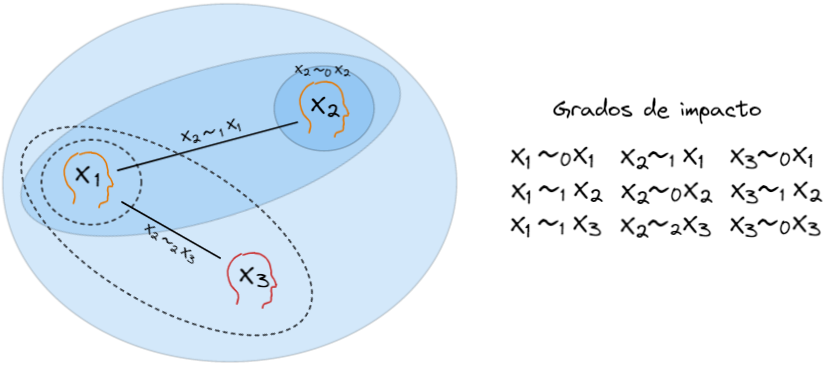
\includegraphics[width=0.75\textwidth]{Imagenes/gradosDiagrama.png}
\end{figure} 
\end{frame}

\begin{frame}{Relaciones entre células: Grados de impacto}
%De la definición de grado de impacto podemos deducir el siguiente resultado:

\textbf{Teorema:} Los grados de impacto de una célula $x$ definen un sistema fundamental de vecindades.

\underline{\textit{Demostración:}}
\begin{enumerate}
    \item Para $x\in\mathcal{L}$ defina recursivamente a los conjuntos $\mathcal{A}_k$ formados por los elementos son los puntos con grado de impacto $k$ con $x$.
    \item Se observa que $A_i\subseteq A_j$ para $0\leq i\leq j$ y de ese modo $A_i\in\mathcal{V}(x)$ para $i=0,1,\cdots,n$
    \item Se comprueba que $A_0$ es la vecindad mínimal de $x$. 
    \begin{enumerate}
        \item $(\subseteq)$ Se toma $y\in U_x$ y se supone que $y\not\thicksim_0 x$ (Contradicción de la definición de $\thicksim_n$).
        \item $(\supseteq)$ Se toma $y\in A_0$ y se afirma que $y\in\bigcap\mathcal{V}(x)$, por lo que $y\in U_x$.
    \end{enumerate}
\end{enumerate}

\textbf{Proposición:} Sea $x\in\mathcal{L}$ una célula y sea $\mathcal{A}$ la familia de conjuntos encajados definidos por el grado de impacto con $x$. Entonces:
\begin{enumerate}
    \item El conjunto $\mathcal{A}$ posee elemento mínimal igual a $A_0$,
    \item $\mathcal{A}$ es un conjunto ordenado finito con el orden de la contenencia, y
    \item $\mathcal{L}$ es un espacio uno-numerable.
\end{enumerate}

%Algo que debemos tener en cuenta es que el grado de impacto por si solo no nos proporciona una medida del impacto que tienen los cambios de estado de células "lejanas" (o de grado de impacto mayor a cero). Estas medidas de impacto se entenderán como la probabilidad de que un cambio de estado afecte a la célula con la que estamos realizando la comparación. De ese modo, las tasas de impacto serán valores entre 0 y 1 que pueden venir dados por cualquier tipo de función que tenga como dominio al conjunto de grados de impacto.
\end{frame}

\begin{frame}{Relaciones entre células: Tasas de impacto}
El grado de impacto por si solo no nos proporciona una medida del impacto que tienen los cambios de estado de células "lejanas" (o de grado de impacto mayor a cero). 

Estas medidas de impacto $P(g)$, se entenderán como la probabilidad de que un cambio de estado afecte a la célula con la que estamos realizando la comparación. De ese modo, las tasas de impacto serán valores entre 0 y 1 que pueden venir dados por cualquier tipo de función que tenga como dominio al conjunto de grados de impacto.

\begin{figure}[h]
  \centering
    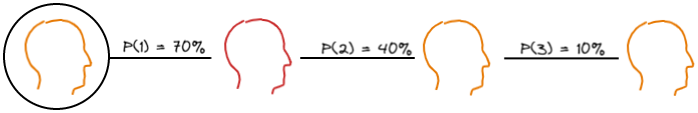
\includegraphics[width=0.75\textwidth]{Imagenes/tasasGrados.png}
\end{figure} 
\end{frame}

\subsection{Reglas de evolución}

\begin{frame}{Reglas de evolución: Niveles de incidencia}
\begin{figure}[h]
  \centering
    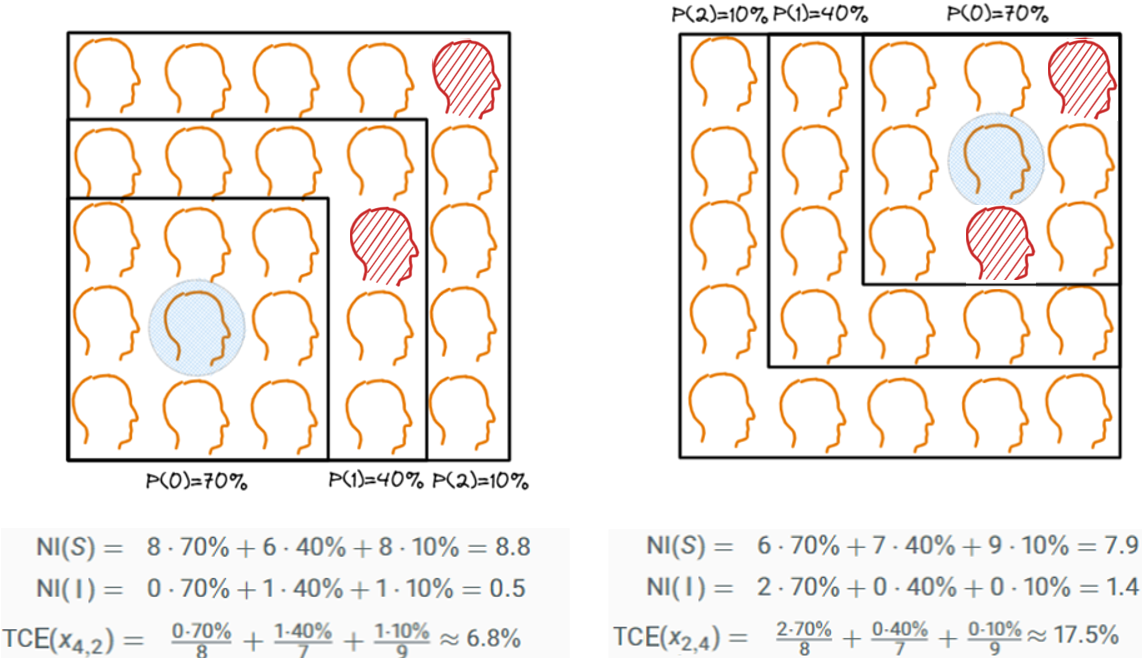
\includegraphics[width=1\textwidth]{Imagenes/nivelesIncidencia.png}
\end{figure}
\end{frame}

\begin{frame}{Reglas de evolución: La regla SI}
Para cada célula en el espacio $\mathcal{L}$ se debe cumplir que:
\begin{itemize}
    \item Si la célula es susceptible a contraer la enfermedad, se mantendrá en ese estado con una probabilidad $i(x)=TCE(x)\cdot\frac{\beta}{\alpha}$, siempre y cuando el nivel de incidencia de la población susceptible sea mayor al de la población infectada.
    \item Si la célula no es susceptible y tampoco está infectada, se mantendrá en el mismo estado.
    \item Se infectará en otro caso.
\end{itemize}

\textbf{Nota:} En la implementación se usó una distribución uniforme para determinar el valor aleatorio usado para el cálculo de la probabilidad, se espera que en futuras investigaciones se profundice en cambios sobre la distribución usada.
\end{frame}

\begin{frame}{Reglas de evolución: Las reglas SIS y SIR}
Para cada célula en el espacio $\mathcal{L}$ se debe cumplir que:
\begin{itemize}
    \item Si es susceptible a contraer la enfermedad, aplique la regla SI.
    \item Si está infectada, se recuperará con una probabilidad $\alpha$ y se mantendrá enferma con una probabilidad $1-\alpha$.
    \item Si es inmune a la enfermedad, se mantiene en ese estado (modelo SIR).
\end{itemize}
\begin{minipage}{0.5\textwidth}
\begin{figure}[h]
  \centering
 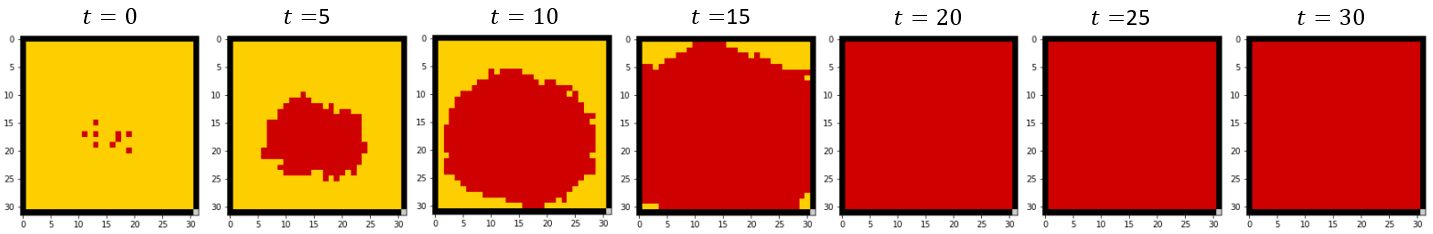
\includegraphics[width=1\textwidth]{Imagenes/sisEn30.PNG}
 \caption{Evolución de la enfermedad - modelo SIS.}
 \label{fig:sisEn30}
\end{figure}
\vspace{-0.5cm}
\begin{figure}[h]
  \centering
 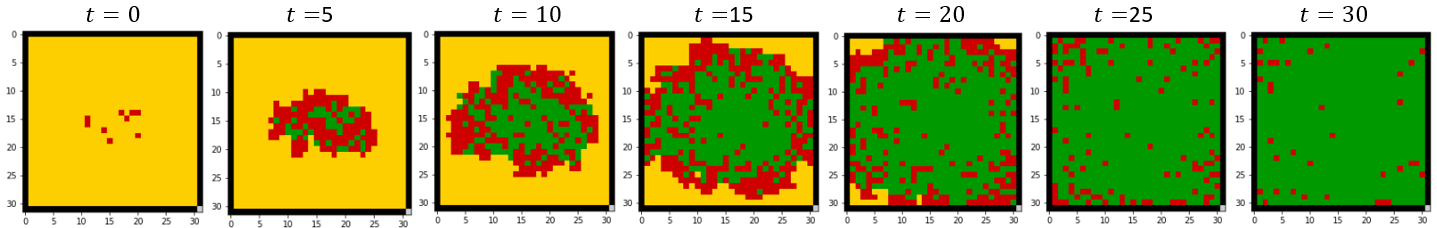
\includegraphics[width=1\textwidth]{Imagenes/sirEn30.PNG}
 \caption{Evolución de la enfermedad - modelo SIR.}
 \label{fig:sirEn30}
\end{figure}
\end{minipage}
\hfill
\begin{minipage}{0.45\textwidth}
\begin{figure}[h]
  \centering
    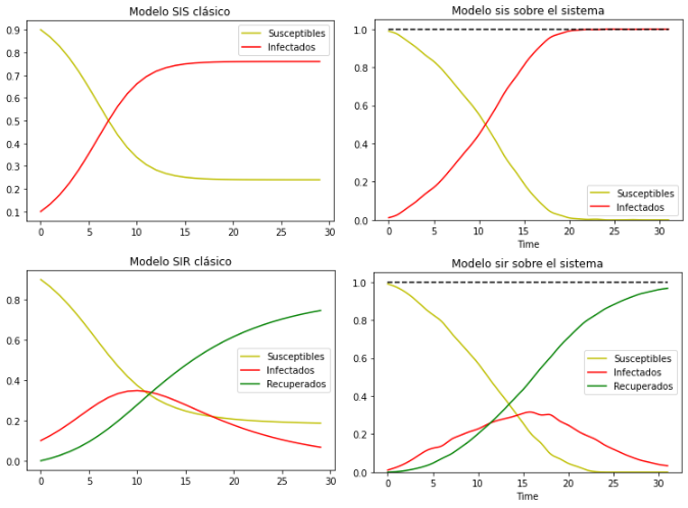
\includegraphics[width=1\textwidth]{Imagenes/solucionesSISySIR1.PNG}
    \caption{Evolución de la enfermedad - modelos clásicos vs reglas de evolución.}
    \label{fig:sirEn30}
\end{figure}
\end{minipage}
\end{frame}

\begin{frame}{Reglas de evolución: Nacimientos y muertes}
\begin{figure}[h]
  \centering
    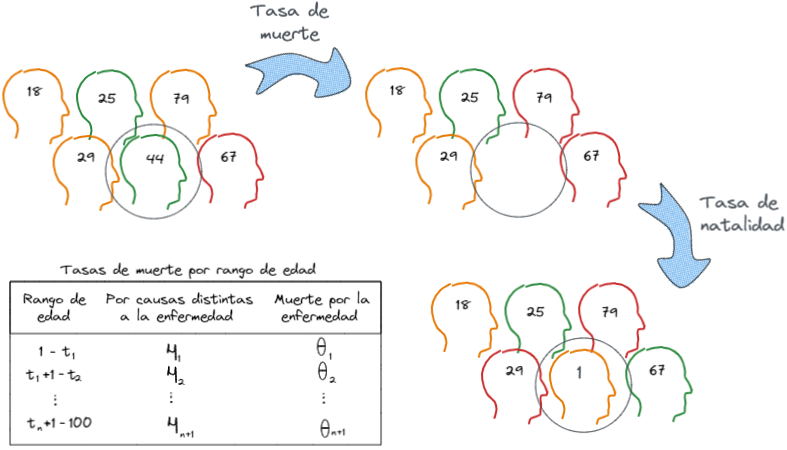
\includegraphics[width=0.85\textwidth]{Imagenes/tasasLetalidad.png}
\end{figure}
\end{frame}

\begin{frame}{Reglas de evolución: Ciclos temporales}
\begin{figure}[h]
  \centering
    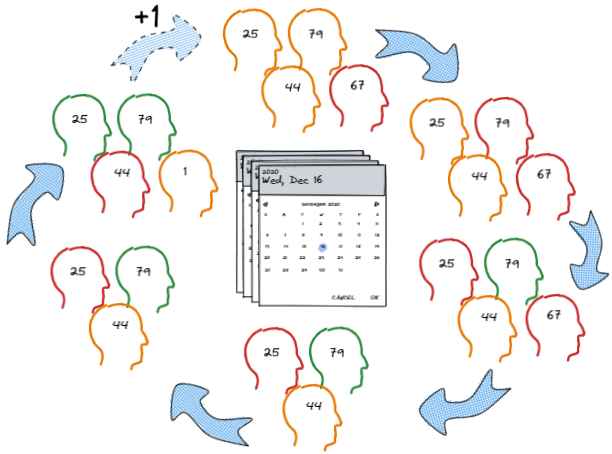
\includegraphics[width=0.8\textwidth]{Imagenes/cicloAnual.png}
\end{figure}
\end{frame}

\section{Ejemplo particular}
\begin{frame}{Ejemplo particular}
\begin{itemize}
    \item \textbf{Escuela (E):} Se sabe que en el pueblo hay 9 niños y 2 profesores.
    \item \textbf{Oficinas (O):} Cuenta con un personal de 16 individuos.
    \item \textbf{Mercado (M):} Se identificaron 8 trabajadores.
    \item \textbf{Hospital (H):} Entre doctores, enfermeros y pacientes se identifica una cantidad de 14 individuos. Para un total de 49 personas en el pueblo.
\end{itemize}
\begin{minipage}{0.48\textwidth}
\begin{figure}[h]
  \centering
    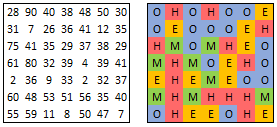
\includegraphics[width=0.7\textwidth]{Imagenes/edadesYOcupaciones.PNG}
    \caption{Edades y ocupaciones en el pueblo.}
    \label{fig:edadesYOcupaciones}
\end{figure}
\end{minipage}
\hfill
\begin{minipage}{0.48\textwidth}
\begin{figure}[h]
  \centering
    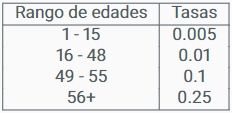
\includegraphics[width=0.65\textwidth]{Imagenes/tasasDeLetalidad_ex_Pueblo.png}
    \caption{Tasas de letalidad de la gripa.}
\end{figure}
\end{minipage}

En el caso de la enfermedad, tomaremos $\alpha=\frac{1}{5}=0.2$ (la gripa dura en promedio 5 días), $\beta=0.3$, tasas de natalidad del $2\%$ y de mortalidad del $0.5\%$. Supondremos inicialmente que la enfermedad inicia en el hospital.
\end{frame}

\begin{frame}{Ejemplo particular}
\begin{figure}[h]
  \centering
    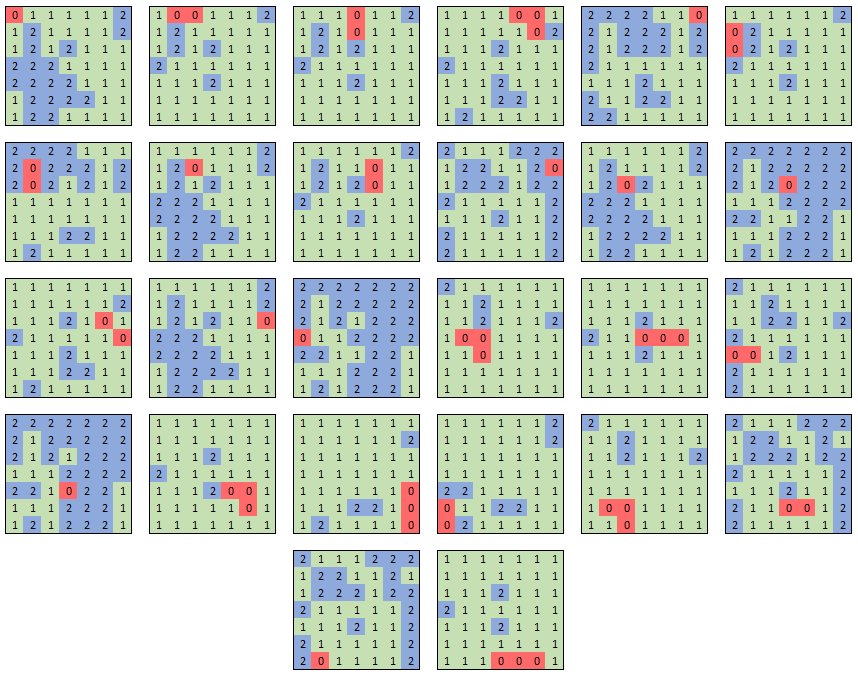
\includegraphics[width=0.8\textwidth]{Imagenes/vecindadesCap4.PNG}
    \caption{Grados de impacto.}
    \label{fig:GradosdeImpactoEX4}
\end{figure}
\end{frame}

\begin{frame}{Ejemplo particular}
Para un periodo de 30 días y las tasas de impacto $P(0)=1,P(1)=0.5$ y $P(2)=0.25$ se tiene el comportamiento descrito en la segunda figura:
\begin{figure}[h]
  \centering
    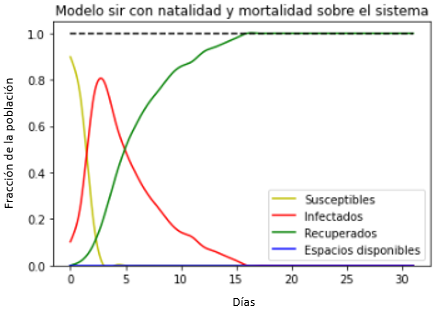
\includegraphics[width=0.5\textwidth]{Imagenes/metricas1.PNG}
    \caption{Cambios de estado con punto de inicio en el hospital.}
    \label{fig:metricas1}
\end{figure}
\end{frame}

\begin{frame}{Ejemplo particular}
En la siguiente figura podremos observar la evolución promedio sobre 100 simulaciones de la enfermedad teniendo en cuenta diferentes tasas de impacto:

\begin{figure}[h]
  \centering
    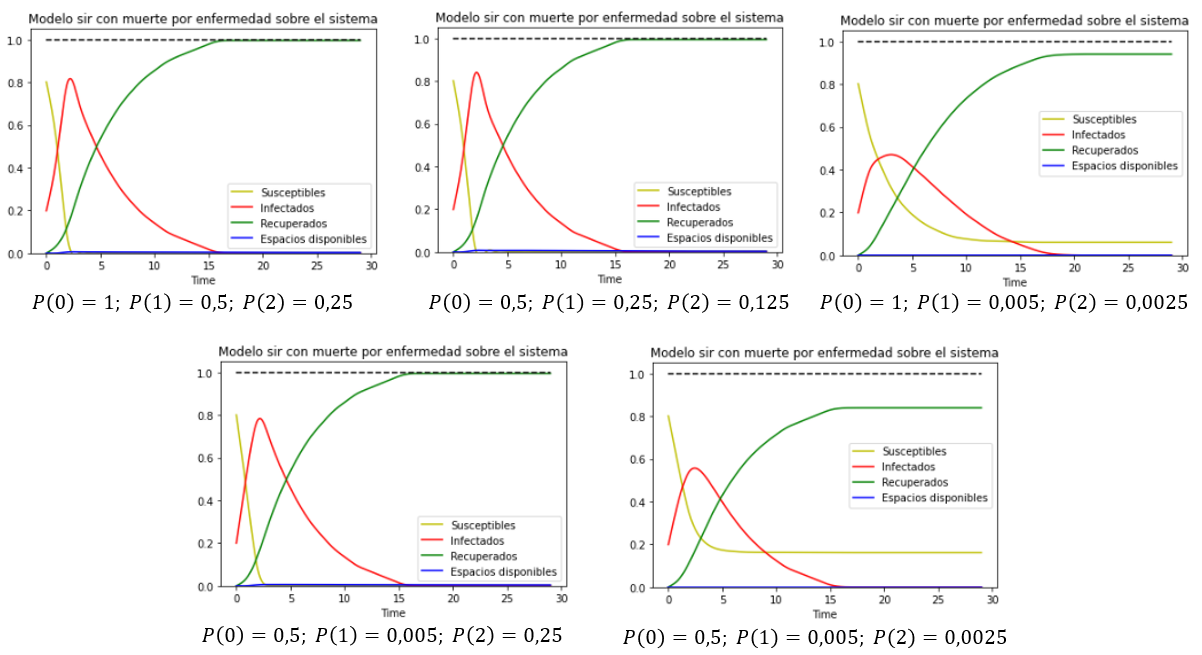
\includegraphics[width=1\textwidth]{Imagenes/comparacionTasasImpacto.PNG}
    \caption{Evolución promedio de la enfermedad tomando distintas tasas de impacto.}
    \label{fig:comparacionTasasdeImpacto}
\end{figure}
\end{frame}

\begin{frame}{Ejemplo particular}
Teniendo en cuenta que el ejemplo anterior muestra que diferentes tasas de impacto afectan a las curvas de evolución del modelo, podemos preguntarnos si ocurre algo similar con diferentes condiciones iniciales. 

\begin{figure}[h]
  \centering
    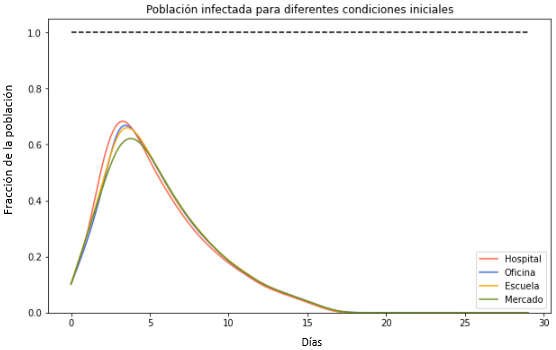
\includegraphics[width=0.5\textwidth]{Imagenes/condicionesIniciales.png}
    \caption{Población infectada por condición inicial.}
    \label{fig:condicionesIniciales}
\end{figure}
\end{frame}

\begin{frame}{Ejemplo particular}
Por otro lado, podemos también preguntarnos si el sistema de vecindades con el que se describen las interacciones, tiene algún tipo de incidencia en el comportamiento de la enfermedad. %Para responder a esta inquietud nos planteamos el escenario que se puede observar en la figura (\ref{fig:comparacionTasasdeImpacto}) en donde se muestra la evolución de la misma enfermedad, sobre un espacio en el que las relaciones entre células se pueden describir a partir de los sistemas de vecindades de Moore y de Von Neumann junto con el escenario planteado durante el presente capítulo. Para los tres escenarios se tomaron las curvas promedio sobre un total de 100 simulaciones.
\begin{figure}[h]
  \centering
    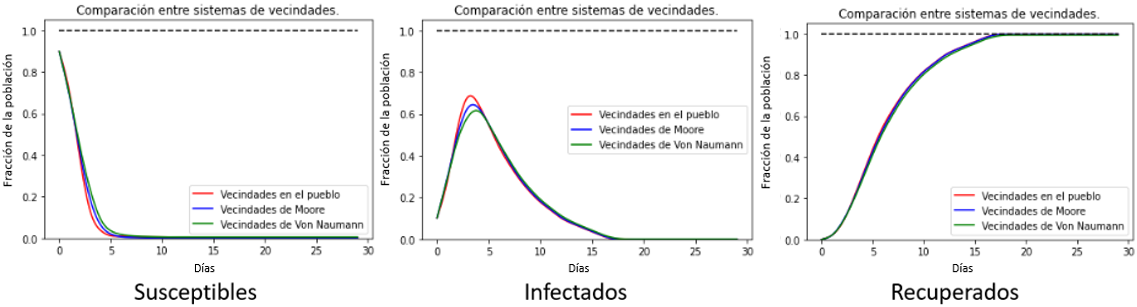
\includegraphics[width=1\textwidth]{Imagenes/comparacionSistemasVecindades.PNG}
    \caption{Evolución promedio de la enfermedad tomando tres sistemas de vecindades.}
    \label{fig:comparacionSistemasDeVecindades}
\end{figure}
\end{frame}

\section{Conclusiones}
\begin{frame}{Conclusiones}
\begin{itemize}
    \item Haciendo uso de las \textbf{propiedades de los autómatas celulares} para describir comportamientos espaciales y de los sistemas fundamentales de vecindades \textbf{es posible modelar las relaciones sociales} de un conjunto de individuos determinado.
    \item Las \textbf{condiciones iniciales} sobre cómo interactúan las células \textbf{no afectan a los puntos de equilibrio} de las curvas que describen el comportamiento de la enfermedad. Sin embargo, como se observa en los ejemplos realizados, los \textbf{cambios en la condición inicial} pueden afectar a la \textbf{velocidad de propagación} de la misma enfermedad.
    \item Se evidencia que limitar y/o reducir la intensidad de las interacciones sociales es una medida efectiva para disminuir los casos de individuos infectados.
\end{itemize}
\end{frame}

\begin{frame}{Conclusiones}
\begin{itemize}
    \item Las reglas y algoritmos propuestos \textbf{permiten visualizar de manera clara e intuitiva a la manera en la que una enfermedad evoluciona dentro de una población}, manteniendo un comportamiento que puede ser descrito en cierta medida por los modelos compartimentales clásicos.
    \item Si bien las reglas planteadas permiten analizar características que no eran posibles con los modelos clásicos, se evidencia una \textbf{limitación} en cuanto a que se asume una \textbf{capacidad máxima de individuos en el sistema.}
    \item La \textbf{metodología} empleada para el diseño e implementación de las reglas de evolución descritas en este trabajo, brindan un camino claro para la definición de reglas que modelen el comportamiento de modelos epidemiológicos más generales.
\end{itemize}
\end{frame}

\section{Referencias}
\begin{frame}[allowframebreaks]{Referencias}
\bibliographystyle{plain} % apalike
\bibliography{BibliMSc}
\end{frame}

\end{document}